\documentclass[10pt]{article}
\usepackage[letterpaper,margin=0.80in,headheight=14pt]{geometry}
\usepackage[T1]{fontenc}
\usepackage{lmodern,microtype}
\usepackage{amsmath,amssymb}
\usepackage{booktabs,array,tabularx,enumitem}
\usepackage[dvipsnames]{xcolor}
\usepackage{hyperref,tikz}
\usetikzlibrary{arrows.meta,positioning}

\definecolor{VALblue}{HTML}{175A6A}
\definecolor{VALpale}{HTML}{EAF4F5}
\definecolor{VALgold}{HTML}{9A6700}
\definecolor{VALgray}{HTML}{4B5563}
\hypersetup{colorlinks=true,linkcolor=VALblue,urlcolor=VALblue,
  hypertexnames=false,
  pdftitle={SCI-VAL Science-Team Rationale v0.1/r0.3},
  pdfauthor={SCI-VAL implementation-blind scientific authorship}}
\setlength{\parindent}{0pt}
\setlength{\parskip}{0.48em}
\setlist{leftmargin=*,nosep}
\renewcommand{\arraystretch}{1.12}
\emergencystretch=3em
\hbadness=10000
\newcommand{\RationaleBox}[2]{\begin{center}\fcolorbox{VALblue}{VALpale}{%
  \parbox{0.92\linewidth}{\textbf{#1}\quad #2}}\end{center}}
\tikzset{valbox/.style={draw=VALblue,thick,rounded corners=2pt,fill=VALpale,
 align=center,minimum height=0.68in,text width=1.55in},
 valarr/.style={-{Latex[length=2.4mm]},thick,draw=VALblue}}

\begin{document}
\raggedbottom

\begin{titlepage}
\thispagestyle{empty}
{\color{VALblue}\rule{\linewidth}{2pt}}\\[0.28in]
{\Huge\bfseries SCI-VAL\\[0.10in]}
{\LARGE Sample and Detector Validity, Flags,\\[0.05in]
and Map Eligibility\\[0.25in]}
{\large\bfseries Producer Facts and Use-Specific Eligibility:\\[0.03in]
Not Final Map Validity\\[0.20in]}
{\huge\color{VALblue}Science-Team Rationale}\par
\vspace{0.34in}
\begin{tabularx}{\linewidth}{@{}p{0.25\linewidth}X@{}}
Scientific contract version & v0.1 \\
Rationale revision & r0.3 \\
Date & 2026-08-24 \\
Input & Exact immutable producer facts/supports plus one exact owner-bound
registered profile \\
Output & Cause-preserving, use-qualified request/applicability/eligibility/
realization record \\
Governing rule & Producers own facts; named-use owners own policy; VAL Core
evaluates; the registry binds but does not author policy \\
Source & Owner-approved r0.3 Core directive plus exact continuing source and
profile registries \\
Status & Content-bound freeze candidate; scientific-owner approval pending;
implementation conformity and validation not assessed \\
\end{tabularx}
\vspace{0.30in}
\RationaleBox{Central claim.}{VAL is an evaluator and registry mechanism, not
a policy author. Registration records who owns a policy, exactly which source
defines it, and how it may be replayed; it never grants scientific authority
to VAL.}

\textbf{Executive abstract.}
A finite value is not necessarily an independent measurement. A retained
value is not necessarily admissible to a fit. A value admitted upstream is not
necessarily projected into a map. SCI-VAL keeps these questions separate by
combining exact producer-owned facts with one exact policy owned by the
scientific use. Its four axes distinguish whether a question was requested,
whether it applies, what its scientific disposition is, and whether an
authoritative decision artifact was realized. Causes remain visible; silence
is not evidence of absence; and an unrelated permission cannot rescue an
applicable exclusion.

V0.1 has one mandatory canonical registered profile:
\texttt{SCI-VAL:independent\_exposure@1}. Its direct-origin rule is a
contract-level scientific invariant: a synthesized or replaced representative
occurrence is not an original independent exposure, and no exception may
redefine it. The continuing registry also binds five exact PTC-owned profiles
for basis fit, loading fit, frozen operator application, ordinary output
retention, and existing tracked-kernel propagation. Generic coefficient/QC
and empirical/simulation identities are explicitly unsupported; MAP remains
unbound. The companion Engineering Conformance Specification is the complete
VAL Core formal authority; the continuing registries bind owner policies and
sources without rewriting that Core.

\vfill
{\color{VALblue}\rule{\linewidth}{2pt}}
\end{titlepage}

\pagenumbering{arabic}
\section{The finite, retained, replaced occurrence}
\label{sec:rat-worked}

Start with one exact detector occurrence. Its stored payload is finite and is
retained. RTC states authoritatively that the exact representative source was
replaced and supplies the replacement cause and source link. The following
questions are not aliases.

\begingroup
\small
\begin{tabularx}{\linewidth}{@{}p{0.27\linewidth}p{0.27\linewidth}X@{}}
\toprule
Question & Profile/authority status & Scientific outcome \\
\midrule
Independent astronomical exposure? & Mandatory canonical profile plus RTC
origin fact & \textbf{Ineligible.} Direct replacement is non-exceptionable;
the cause remains visible. \\
Receive a frozen operator? & Exact
\nolinkurl{SCI-PTC:operator_application@1} profile; required group-time facts are
not supplied by this worked case & \textbf{Decision unavailable here.} Direct
replacement is not itself an application veto; complete operator facts would
decide this separate use. \\
Remain in an ordinary PTC output? & Exact
\nolinkurl{SCI-PTC:output_retention@1} profile plus RTC replacement fact &
\textbf{Ineligible.} Direct replacement is excluded from ordinary PTC
science-signal support even if a numerical value was calculated. \\
Display for diagnosis? & Purely informational display; no admission or
decision role requested & No eligibility proposition. The value may remain
visible with replacement provenance and no stronger claim. \\
Enter PTC basis fitting? & Exact
\nolinkurl{SCI-PTC:basis_fit_admission@1} profile plus RTC replacement fact &
\textbf{Ineligible.} The occurrence teaches neither ordinary centering nor
the PCA basis. \\
Enter PTC loading fitting? & Exact
\nolinkurl{SCI-PTC:loading_fit_admission@1} profile plus RTC replacement fact &
\textbf{Ineligible.} Loading permission remains distinct from basis
permission. \\
Enter generic coefficient/QC estimation? & Broad profile identity explicitly
unsupported & No present proposition is available for VAL to evaluate; a
future diagnostic with decision authority needs its own exact profile. \\
Pass MAP upstream admission? & MAP boundary known; exact profile absent &
Decision unavailable. Even eligibility would not prove projection,
contribution, support, or final validity. \\
\bottomrule
\end{tabularx}
\endgroup

\RationaleBox{Why one flag fails.}{This occurrence is finite and upstream
retained, but directly replaced and therefore ineligible for independent
exposure, ordinary PTC basis/loading influence, and ordinary PTC output
retention. Exact frozen-operator application remains a separate question;
informational display asserts no eligibility proposition; MAP remains
unbound. A single good/bad bit loses the scientific question, owner, and
reason.}

The independent-exposure result is not a hidden VAL policy. The exact
scientific owner is recorded in the immutable registry binding; the
\texttt{SCI-VAL} namespace identifies the registry package, not the policy
owner. VAL checks and evaluates that immutable binding. A policy that tries
to override the non-exceptionable origin rule is invalid. Hypothetical complete
future profiles remain unavailable until their exact owner,
source, domain, restrictions, and compatibility are registered; a name alone
conveys no permission. ``Would be eligible'' is therefore a conditional
statement about a complete future binding, never a present decision. The
invalid-origin override yields decision
unavailable with a policy-invalid reason, never eligible.

\clearpage
\section{Four authorities must stay separate}
\label{sec:rat-authority}

The scientific chain has four distinct authorities. A producer describes what
happened and what its own operation supports. The owner of the named use says
which of those facts matter for that exact question. VAL checks identities and
executes the supplied rule. The consumer performs its numerical action and
owns the final product claim.

\begin{center}
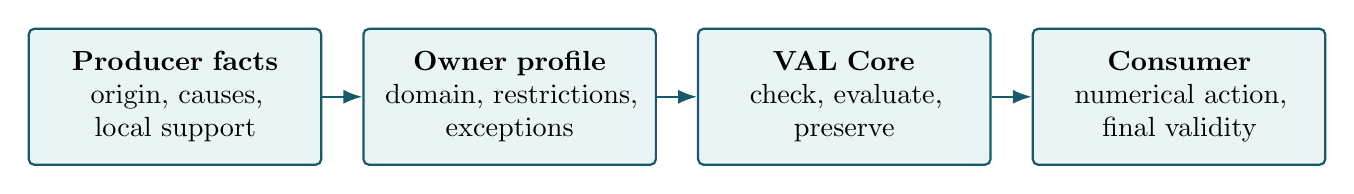
\begin{tikzpicture}[node distance=0.20in]
\node[valbox,text width=1.37in] (facts) {\textbf{Producer facts}\\origin, causes,\\local support};
\node[valbox,text width=1.37in,right=of facts] (profile) {\textbf{Owner profile}\\domain,
restrictions,\\exceptions};
\node[valbox,text width=1.37in,right=of profile] (val) {\textbf{VAL Core}\\check, evaluate,\\preserve};
\node[valbox,text width=1.37in,right=of val] (consumer) {\textbf{Consumer}\\numerical action,\\final validity};
\draw[valarr] (facts)--(profile);
\draw[valarr] (profile)--(val);
\draw[valarr] (val)--(consumer);
\end{tikzpicture}
\end{center}

The Profile Registry sits alongside this chain. It binds an immutable profile
identity to the actual scientific owner, source version or digest, domain,
restrictions, exception permissions, and compatibility rules. It does not
copy the policy into VAL ownership. A reserved name with no exact binding is
not a usable policy.

\begin{center}
\begin{tabularx}{\linewidth}{@{}p{0.21\linewidth}Xp{0.30\linewidth}@{}}
\toprule
Authority & Owns & Cannot infer \\
\midrule
Producer & Facts, causes, explicit negative assertions, producer-local
composites and influence & A downstream use policy \\
Named-use owner & Applicability, restrictions, exceptions, aggregation,
thresholds, failure scope & Facts owned by another producer \\
Profile Registry & Immutable owner/source/domain/compatibility binding & A
missing predicate or owner \\
VAL Core & Shared logic, provenance, deterministic evaluation & A PTC or MAP
policy, threshold, or universal flag \\
Consumer & Estimator action and final product validity & Promotion of an
invalid parent because a descendant is finite \\
\bottomrule
\end{tabularx}
\end{center}

This split is why PTC owns basis-fit, loading-fit, application, output, and
coefficient/QC supports separately, while MAP owns upstream admission,
projection, numerical contribution, support, response/covariance, coaddition,
and final validity separately. VAL can evaluate a registered profile for one
of those questions; it cannot collapse the questions or author the answer.

\clearpage
\section{Four axes, open-world facts, and no-rescue logic}
\label{sec:rat-axes}

Every decision carries four independent answers.

\begin{center}
\begin{tabularx}{\linewidth}{@{}p{0.17\linewidth}p{0.31\linewidth}X@{}}
\toprule
Axis & Values & Question answered \\
\midrule
Request & requested / not requested & Was an authoritative evaluation asked
for? \\
Applicability & applicable / inapplicable / unknown & Is this profile defined
for this object and domain? \\
Eligibility & eligible / ineligible / decision unavailable & What can the
known facts establish for this exact use? \\
Realization & realized / incomplete / failed / not produced & Does an
authoritative decision artifact exist? \\
\bottomrule
\end{tabularx}
\end{center}

If no request was made, no eligibility proposition is invented. If the
profile is known not to apply, there is likewise no eligibility proposition.
If the scientific question is well defined but a required fact is unresolved,
the correct result is decision unavailable. A failed output artifact is a
failure of realization, not a new scientific disposition.

Facts are open-world. An authoritative producer can say true or explicitly
false; information can also be unknown or conflicting. Silence about a cause
is unknown. It becomes authoritative absence only when the owning producer
declares the relevant cause family complete and explicitly asserts absence.

A conflict in identity, parentage, profile authority, applicability, or
another structural-gate fact prevents the scientific question from being
established: applicability is unknown and the decision is unavailable. Once
the domain is established, a non-gating conflict is preserved as unresolved
evidence rather than promoted to a structural failure.

Once the structural question is established, applicable restrictions compose
conservatively:
\[
\begin{array}{ccl}
\text{one known exclusion} &+& \text{any unrelated permission, unknown, or conflict}
\quad\Longrightarrow\quad \text{ineligible},\\[0.2em]
\text{no exclusion} &+& \text{at least one required unknown or conflict}
\quad\Longrightarrow\quad \text{decision unavailable},\\[0.2em]
\text{all required permissions known} &&
\quad\Longrightarrow\quad \text{eligible}.
\end{array}
\]

A permitted exception can neutralize only the exact exceptionable restriction
named by the same owner-bound profile. It never erases the underlying cause,
and it cannot touch the independent-exposure origin invariant. Unknown or
conflicting exception applicability cannot neutralize the restriction; the
underlying exclusion remains and the conflict is preserved. A permission is a
use-specific disposition, not a new cause.

\clearpage
\section{Direct origin, inherited influence, and immutable generations}
\label{sec:rat-influence}

Direct origin and inherited influence answer different causal questions. A
representative occurrence synthesized or replaced upstream is directly not an
original independent exposure. A different occurrence may only be influenced
by that source through an operator. That edge can be exact and confirmed, or
conservative and merely possible. A conservative envelope may deliberately
overstate influence; it must never be relabeled exact.

\begin{center}
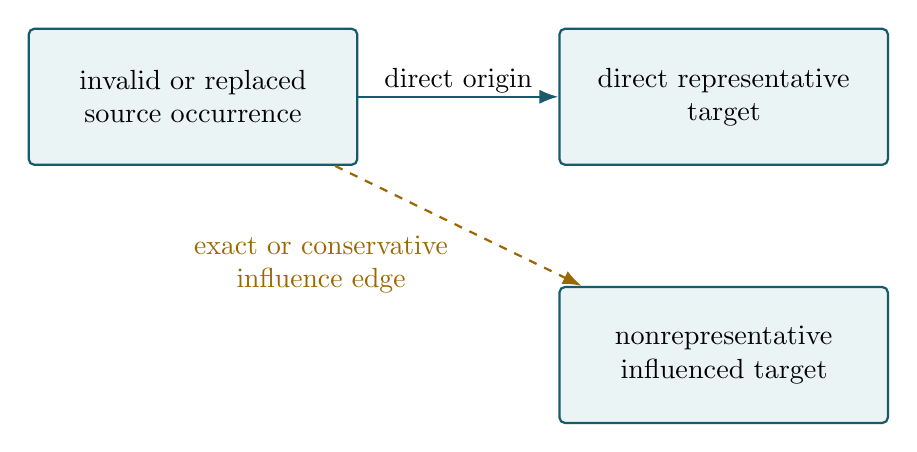
\begin{tikzpicture}[node distance=0.45in]
\node[valbox,text width=1.55in] (source) {invalid or replaced\\source occurrence};
\node[valbox,text width=1.55in,right=1.0in of source] (rep) {direct representative\\target};
\node[valbox,text width=1.55in,below=0.60in of rep] (other) {nonrepresentative\\influenced target};
\draw[valarr] (source)-- node[above,fill=white,inner sep=1pt]{direct origin} (rep);
\draw[valarr,dashed,VALgold] (source)-- node[below left,align=center,text=VALgold]{exact or conservative\\influence edge} (other);
\end{tikzpicture}
\end{center}

The direct representative link activates the independent-exposure invariant.
The nonrepresentative edge has no universal downstream disposition. Its use
owner may permit it, exclude it, request review, or state scientific
unavailability. Review is action metadata, not a fourth eligibility state,
and no choice changes the producer-owned causal record.

Decisions are snapshots. Later information creates a later generation:
\[
\text{facts}_k\;\longrightarrow\;\text{VAL decision}_k
\;\longrightarrow\;\text{consumer action}_k
\;\longrightarrow\;\text{facts}_{k+1}.
\]
The later generation cannot rewrite what the earlier consumer knew or did.
This is especially important for staged PTC decisions. A later output reject
does not rewrite basis-fit membership; a coefficient/QC decision does not
rewrite a loading fit; only the PTC owner can decide that a changed fit support
requires refitting.

Source and profile changes follow the same rule. A new source digest,
exception resolution, profile version, or compatibility binding creates a new
replay identity. ``Use the current policy'' is not reproducible scientific
provenance.

\clearpage
\section{Aggregation is a new scientific proposition}
\label{sec:rat-aggregation}

An aggregate such as a detector-level rejected fraction is not a bare number.
It has its own registered profile identity, scientific owner, version,
applicability domain, operator, threshold, and propagation authority. That
aggregate profile also binds the exact atomic source-profile identity from
which its inputs were produced. It cannot reuse the atomic profile identity
or masquerade as another atomic occurrence. Its owner must additionally state
the exact occurrence population and time support, counts on all four axes,
denominator, treatment of missing decisions, boundary polarity, uncertainty,
and whether the result is advisory or binding.

For example, the atomic profile might be
\texttt{SCI-VAL:independent\_exposure@1}, while a future aggregate could be
\texttt{SCI-PTC:detector\_independent\_exposure\_fraction@1}. The latter name
is hypothetical and unavailable here; only a complete immutable record from
its actual owner could make that aggregate proposition evaluable.

Base v0.1 adds a strict compatibility rule. Every atomic decision must share
the same exact profile identity and version, lifecycle stage, object type, and
applicability domain, and the aggregate profile must name that exact compatible
atomic source profile. ``Eighty percent eligible'' is meaningless if some inputs
were judged for diagnostic display and others for independent exposure. A
heterogeneous aggregate is unavailable unless a future owner-approved
transformation maps all inputs to one common proposition; VAL supplies no such
transformation.

\begin{center}
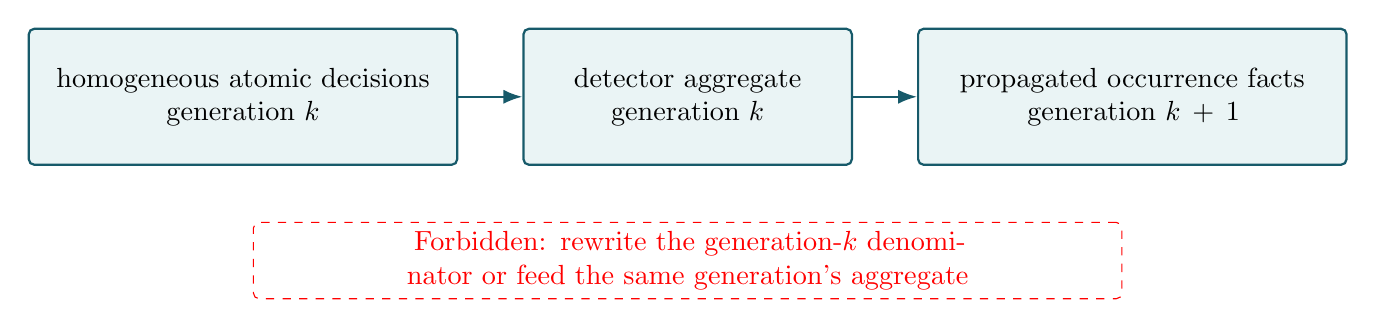
\begin{tikzpicture}[node distance=0.32in]
\node[valbox,text width=2.05in] (atomic) {homogeneous atomic decisions\\generation $k$};
\node[valbox,text width=1.55in,right=of atomic] (agg) {detector aggregate\\generation $k$};
\node[valbox,text width=2.05in,right=of agg] (prop) {propagated occurrence facts\\generation $k+1$};
\draw[valarr] (atomic)--(agg);
\draw[valarr] (agg)--(prop);
\node[draw=red,dashed,rounded corners=2pt,text=red,align=center,
 text width=4.25in,below=0.28in of agg] (ban)
 {Forbidden: rewrite the generation-$k$ denominator or feed the same
 generation's aggregate};
\end{tikzpicture}
\end{center}

Reverse propagation therefore creates new producer facts and new decisions at
generation $k+1$. It cannot alter the generation-$k$ decisions that formed its
own denominator. Any iterative detector classifier needs separately approved
bounds and a stop rule.

An empty or unknown denominator is never a valid zero fraction. Permuting the
same homogeneous multiset cannot change the result. Partitioned and
unpartitioned evaluation are equivalent only when the aggregation owner has
declared a sufficient summary and associative combine rule for the exact
missing, threshold, boundary, and uncertainty semantics.

\clearpage
\section{Profiles, source bindings, response, and uncertainty}
\label{sec:rat-profiles}

Package-qualified names stop broad vocabulary from merging different
scientific questions. V0.1 reserves distinct PTC names for basis-fit
admission, loading-fit admission, frozen-operator application, output
retention, coefficient/QC population, response companion, and
empirical/simulation population. MAP uses
\texttt{SCI-MAP:map\_upstream\_admission}, not the ambiguous former phrase
\texttt{analysis\_or\_gridding\_contribution}. A reserved name still supplies
no policy.

The table below is the \textbf{r0.3 registry snapshot}.
\texttt{SOURCE\_BINDING\_REGISTER.md} is the continuing authority, so a later
adjacent binding update does not by itself rewrite VAL Core.

\begin{center}
\small
\begin{tabularx}{\linewidth}{@{}p{0.13\linewidth}p{0.24\linewidth}X@{}}
\toprule
Source & Exact binding used here & Availability consequence \\
\midrule
RTC & v0.1/r0.9 frozen authority plus sanitized boundary & Representative
origin and influence meanings are bound; changed origin semantics require a
new compatibility review. \\
CAL & v0.1/r0.3 architecture-frozen rationale; scientific authority open &
Boundary meanings are conditional; missing numerical authority remains
unavailable. \\
PTC & v0.1/r0.4 frozen authority as recorded in the program index plus
sanitized boundary & Stage meanings are bound; exact PTC policy profiles are
not supplied by VAL. \\
MAP & v0.1/r0.3 house rationale; scientific authority open; accepted F010/ADR
boundary & Boundary separation is bound; exact MAP upstream-admission profile
remains unavailable. \\
\bottomrule
\end{tabularx}
\end{center}

Response and uncertainty availability are typed facts, not numeric zero or
identity. The use owner assigns exactly one role:

\begin{center}
\small
\begin{tabularx}{\linewidth}{@{}p{0.25\linewidth}X@{}}
\toprule
Role & Scientific consequence \\
\midrule
\texttt{structural\_gate} & Without authoritative satisfaction,
applicability is unknown and the decision is unavailable. \\
\texttt{required\_permission} & Availability is required; known failure
excludes, while unknown or conflict is unresolved. \\
\texttt{decisive\_exclusion} & Authoritative failure excludes; unknown or
conflict is unresolved. \\
\texttt{advisory} & The state is preserved but cannot determine eligibility. \\
\bottomrule
\end{tabularx}
\end{center}

VAL executes that role but does not choose it. Invalid payloads are excluded
before arithmetic. If an admitted required payload is then found non-finite,
the declared operation fails or becomes unavailable at the owner-defined
scope. Finiteness never repairs missing calibration, response, uncertainty,
parent, or policy authority.

\RationaleBox{Availability is not rejection.}{An unavailable profile, source,
response, or required fact yields an explicit inability to decide. It is not
silently interpreted as clean, zero, identity, or eligible.}

\clearpage
\section{What would test the contract, and what remains deferred}
\label{sec:rat-validation}

The engineering specification states 49 normative requirements and 24
falsifiable predictions. They define future checks; they do not report that
an implementation has passed.

\begin{center}
\begin{tabularx}{\linewidth}{@{}p{0.24\linewidth}Xp{0.28\linewidth}@{}}
\toprule
Evidence layer & Question it could answer & Not established by this draft \\
\midrule
Logical fixtures & Does the evaluator preserve axes, causes, registry
bindings, truth-table outcomes, and deterministic replay? & Present
implementation conformity \\
Representation checks & Does a chosen schema preserve every required
distinction and immutable identity? & Scientific correctness of thresholds \\
End-to-end scientific tests & Do known injections, source changes, aggregate
partitions, and propagation generations behave as predicted? & Observational
performance without data \\
Observational validation & Do real reductions meet preregistered scientific
criteria? & Production readiness by itself \\
Operations review & Are evidence, failure handling, monitoring, and ownership
adequate for use? & Authority to change the scientific contract \\
\bottomrule
\end{tabularx}
\end{center}

No general SCI-VAL scientific question remains open from the six first-pass
derivation items. Science now fixes the partial eligibility proposition,
conflict precedence, review as action metadata, the four response/uncertainty
roles, exception lineage, and the conservative aggregation rule. Exact
serialization of an uninstantiated eligibility slot and review metadata is
engineering-deferred. Sufficient summaries, associative combine rules, and
partition equivalence remain profile-local declarations, not VAL defaults.

The main falsifiers are concrete. A direct replacement admitted as independent
exposure, a reserved name yielding eligibility, a mixed-profile aggregate
being treated as a valid fraction, propagation rewriting its own denominator,
a changed source digest replaying as the old policy, or MAP upstream admission
being promoted to actual contribution would each violate this contract.

\RationaleBox{Present status.}{This r0.3 revision resolves the general
architecture, authority, naming, aggregate-identity, conflict, role, feedback,
and source-binding questions assigned to this surgical round. It does not
freeze SCI-VAL, assess an
implementation, validate observational behavior, or authorize production
use.}

\textbf{Reading rule.} The companion Engineering Conformance Specification is
the complete formal authority. This rationale explains that authority in
science-team language and cannot waive a requirement or convert an unavailable
state into a pass.

\end{document}
